% =====================================================================
%  Student architecture — NAFNet w16_sidd, exactly as built.
%
%  Traced from src/models/nafnet.py (NAFBlock.forward, NAFNet.forward) and
%  src/models/norms.py. Nothing is idealised: channel counts, expansion
%  factors, the zero-initialised residual scales beta/gamma, the ADDITIVE skip
%  connections (x + skip, not concatenation) and the three distinct
%  normalisation variants are what the code constructs.
%
%  Compile:  pdflatex student_block.tex
% =====================================================================
\documentclass[tikz,border=6pt]{standalone}
\usepackage{tikz}
\usetikzlibrary{positioning,arrows.meta,calc,fit,backgrounds}

% ---- palette, echoing the NAFNet paper's figure ----------------------
\definecolor{cNorm} {RGB}{244,196,148}   % normalisation      (orange)
\definecolor{cConv} {RGB}{ 74,134,232}   % pointwise conv     (blue)
\definecolor{cDConv}{RGB}{182,215,168}   % depthwise conv     (green)
\definecolor{cGate} {RGB}{162,215,216}   % SimpleGate         (teal)
\definecolor{cAttn} {RGB}{234,153,153}   % channel attention  (red)
\definecolor{cClamp}{RGB}{255,229,153}   % clamp              (yellow)
\definecolor{cBG}   {RGB}{229,229,229}

\tikzset{
  op/.style     = {draw=black!55, rounded corners=1pt, minimum width=25mm,
                   minimum height=5.4mm, font=\scriptsize, inner sep=1.6pt,
                   align=center},
  norm/.style   = {op, fill=cNorm},
  conv/.style   = {op, fill=cConv, text=white},
  dconv/.style  = {op, fill=cDConv},
  gate/.style   = {op, fill=cGate},
  attn/.style   = {op, fill=cAttn},
  clamp/.style  = {op, fill=cClamp},
  flow/.style   = {-{Latex[length=1.6mm]}, black!70, line width=0.45pt},
  oplus/.style  = {circle, draw=black!70, inner sep=0pt, minimum size=3.2mm,
                   font=\tiny},
  scal/.style   = {font=\scriptsize\itshape, text=black!70},
  blkcap/.style = {font=\small, align=center},
}

% =====================================================================
%  \nafblock{<x offset>}{<caption>}{<norm label>}{<1 = extra clamp>}{<clamp>}
%
%  One NAFBlock column. The ONLY difference between our variants is which
%  normalisation sits at norm1/norm2 — every conv, gate and residual is
%  identical. That is the whole point of the ablation, so the figure is
%  generated from one macro rather than drawn four times.
% =====================================================================
\newcommand{\nafblock}[5]{%
  \begin{scope}[shift={(#1,0)}]
    %% ---------------- branch 1: gated depthwise conv + SCA ------------
    \node[norm] (n1) at (0,0) {#3};
    \def\prev{n1}%
    \ifnum#4=1
      \node[clamp] (c1) [below=2.4mm of n1] {#5};
      \draw[flow] (n1) -- (c1);
      \def\prev{c1}%
    \fi
    \node[conv]  (k1) [below=2.4mm of \prev] {$1{\times}1$ conv, $c\!\to\!2c$};
    \draw[flow] (\prev) -- (k1);
    \node[dconv] (k2) [below=2.4mm of k1]  {$3{\times}3$ dconv, groups${=}2c$};
    \node[gate]  (g1) [below=2.4mm of k2]  {SimpleGate, $2c\!\to\!c$};
    \node[attn]  (sa) [below=2.4mm of g1]  {SCA};
    \node[conv]  (k3) [below=2.4mm of sa]  {$1{\times}1$ conv, $c\!\to\!c$};
    \node[oplus] (a1) [below=4.0mm of k3]  {$+$};
    \node[scal] [right=1.0mm of a1] {$\beta$};
    \draw[flow] (k1) -- (k2);
    \draw[flow] (k2) -- (g1);
    \draw[flow] (g1) -- (sa);
    \draw[flow] (sa) -- (k3);
    \draw[flow] (k3) -- (a1);

    %% ---------------- branch 2: gated feed-forward --------------------
    \node[norm] (n2) [below=4.0mm of a1] {#3};
    \def\prevb{n2}%
    \ifnum#4=1
      \node[clamp] (c2) [below=2.4mm of n2] {#5};
      \draw[flow] (n2) -- (c2);
      \def\prevb{c2}%
    \fi
    \node[conv]  (k4) [below=2.4mm of \prevb] {$1{\times}1$ conv, $c\!\to\!2c$};
    \draw[flow] (\prevb) -- (k4);
    \node[gate]  (g2) [below=2.4mm of k4] {SimpleGate, $2c\!\to\!c$};
    \node[conv]  (k5) [below=2.4mm of g2] {$1{\times}1$ conv, $c\!\to\!c$};
    \node[oplus] (a2) [below=4.0mm of k5] {$+$};
    \node[scal] [right=1.0mm of a2] {$\gamma$};
    \draw[flow] (a1) -- (n2);
    \draw[flow] (k4) -- (g2);
    \draw[flow] (g2) -- (k5);
    \draw[flow] (k5) -- (a2);

    %% ---------------- residual bypasses -------------------------------
    \coordinate (bin) at ($(n1)+(0,8mm)$);
    \draw[flow] (bin) -- (n1);
    \draw[flow] (bin) -- ++(-18mm,0) |- (a1);
    \draw[flow] ($(a1)+(0,-2.0mm)$) -- ++(-18mm,0) |- (a2);
    \draw[flow] (a2) -- ++(0,-8mm);

    % Captions on ONE baseline: the clamped columns carry two extra boxes, so
    % an offset relative to (a2) would stagger them.
    \ifnum#4=1 \def\capdrop{-15mm}\else \def\capdrop{-30.6mm}\fi
    \node[blkcap] at ($(a2)+(0,\capdrop)$) {#2};
  \end{scope}}

% ---------------------------------------------------------------------
%  U-Net stage box:  \stage{<name>}{<blocks>}{<channels>}{<fill>}
% ---------------------------------------------------------------------
\tikzset{
  stg/.style   = {draw=black!55, rounded corners=1.5pt, minimum width=17mm,
                  minimum height=8.5mm, font=\scriptsize, align=center},
  resamp/.style= {draw=black!45, fill=black!8, rounded corners=1pt,
                  minimum width=13mm, minimum height=5mm, font=\tiny,
                  align=center},
  skipl/.style = {-{Latex[length=1.5mm]}, black!55, dashed, line width=0.45pt},
}

\begin{document}

% =====================================================================
%  FIGURE 1 — the three normalisation variants of our NAFBlock
%
%  (a) is NAFNet as published, kept as the reference column.
%  (b),(c),(d) are what w16_sidd actually instantiates, stage by stage.
% =====================================================================
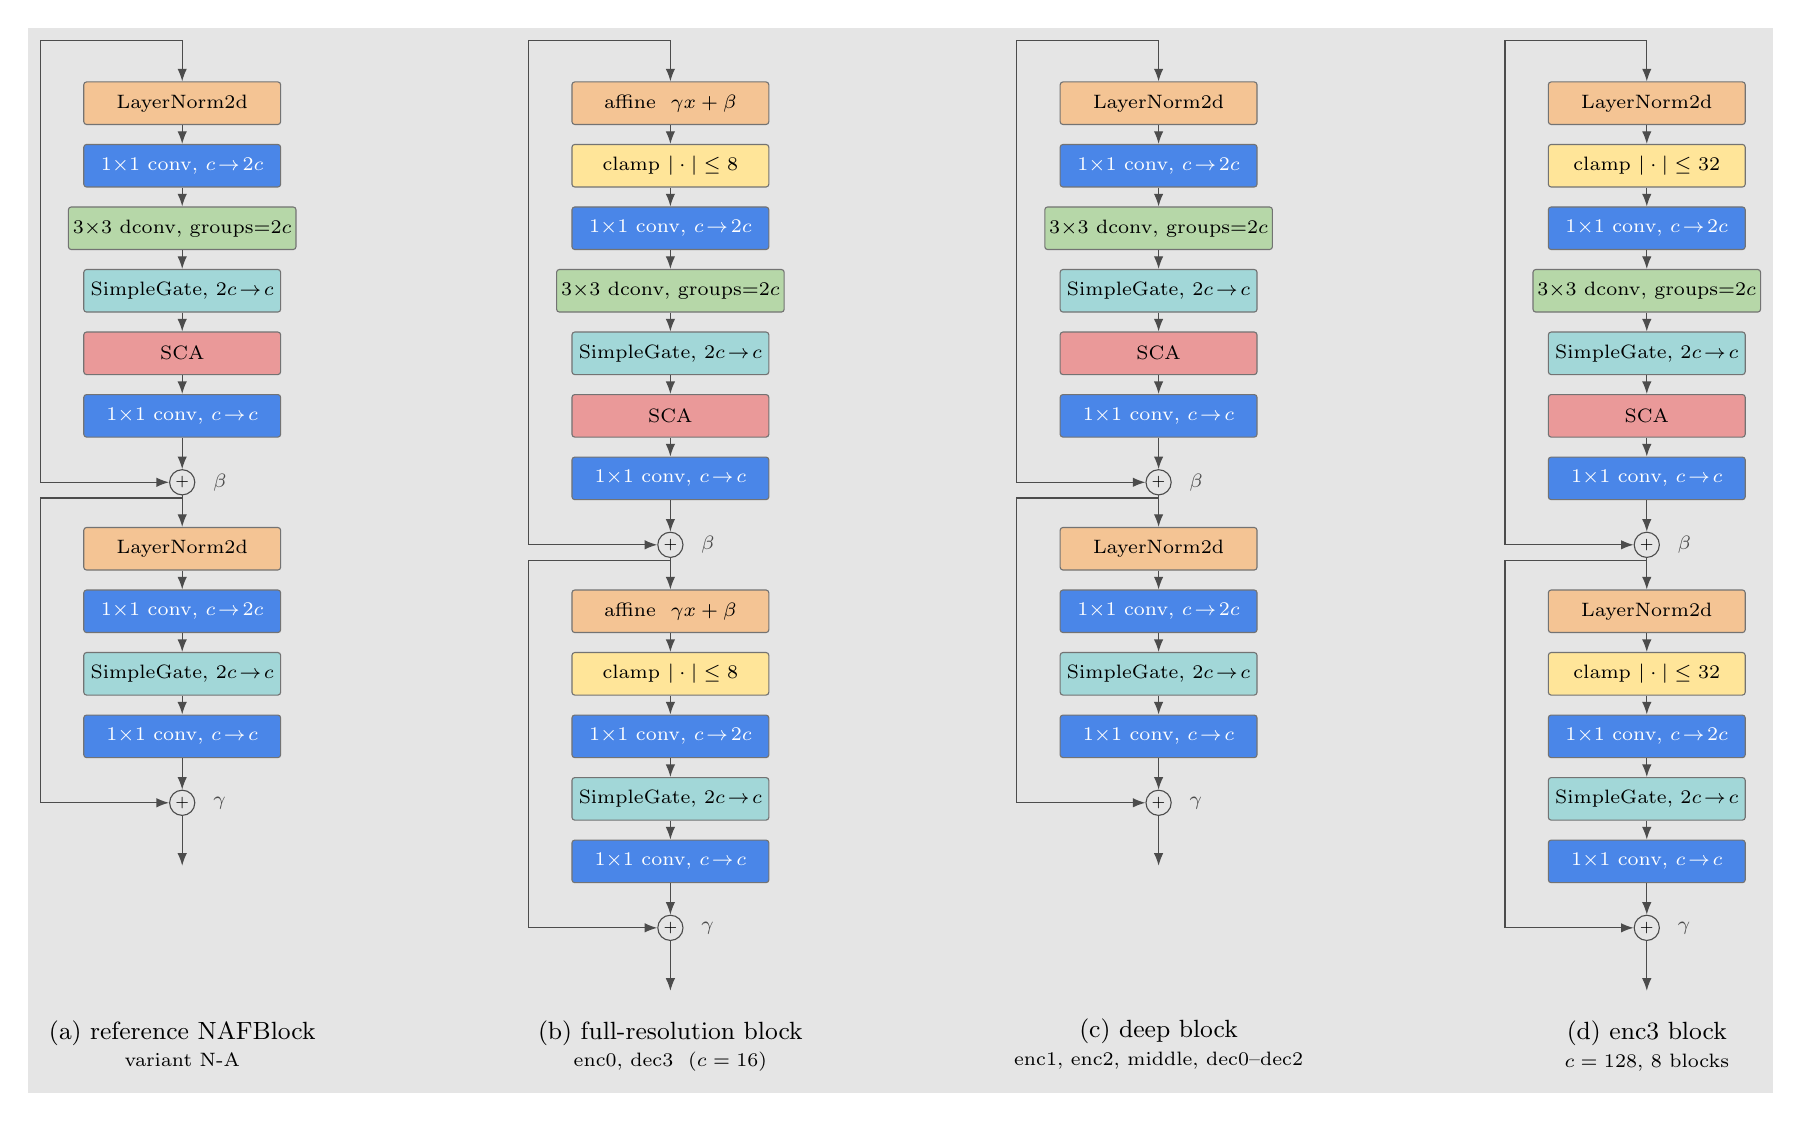
\begin{tikzpicture}[background rectangle/.style={fill=cBG},
                    show background rectangle]

  \nafblock{0}{(a) reference NAFBlock\\[-1pt]\scriptsize variant N-A}%
              {LayerNorm2d}{0}{}

  \nafblock{6.2}{(b) full-resolution block\\[-1pt]%
                 \scriptsize enc0, dec3 \ ($c=16$)}%
              {affine \ $\gamma x+\beta$}{1}{clamp $|\cdot|\le 8$}

  \nafblock{12.4}{(c) deep block\\[-1pt]%
                  \scriptsize enc1, enc2, middle, dec0--dec2}%
              {LayerNorm2d}{0}{}

  \nafblock{18.6}{(d) enc3 block\\[-1pt]%
                  \scriptsize $c=128$, 8 blocks}%
              {LayerNorm2d}{1}{clamp $|\cdot|\le 32$}

\end{tikzpicture}

% =====================================================================
%  FIGURE 2 — the whole student, w16_sidd (7,371,923 parameters)
%
%  Stage block counts [2,2,4,8] / 12 / [2,2,2,2] and width 16 are the
%  configuration in configs/train/*.yaml. Colours mark which normalisation
%  each stage uses, matching Figure 1.
% =====================================================================
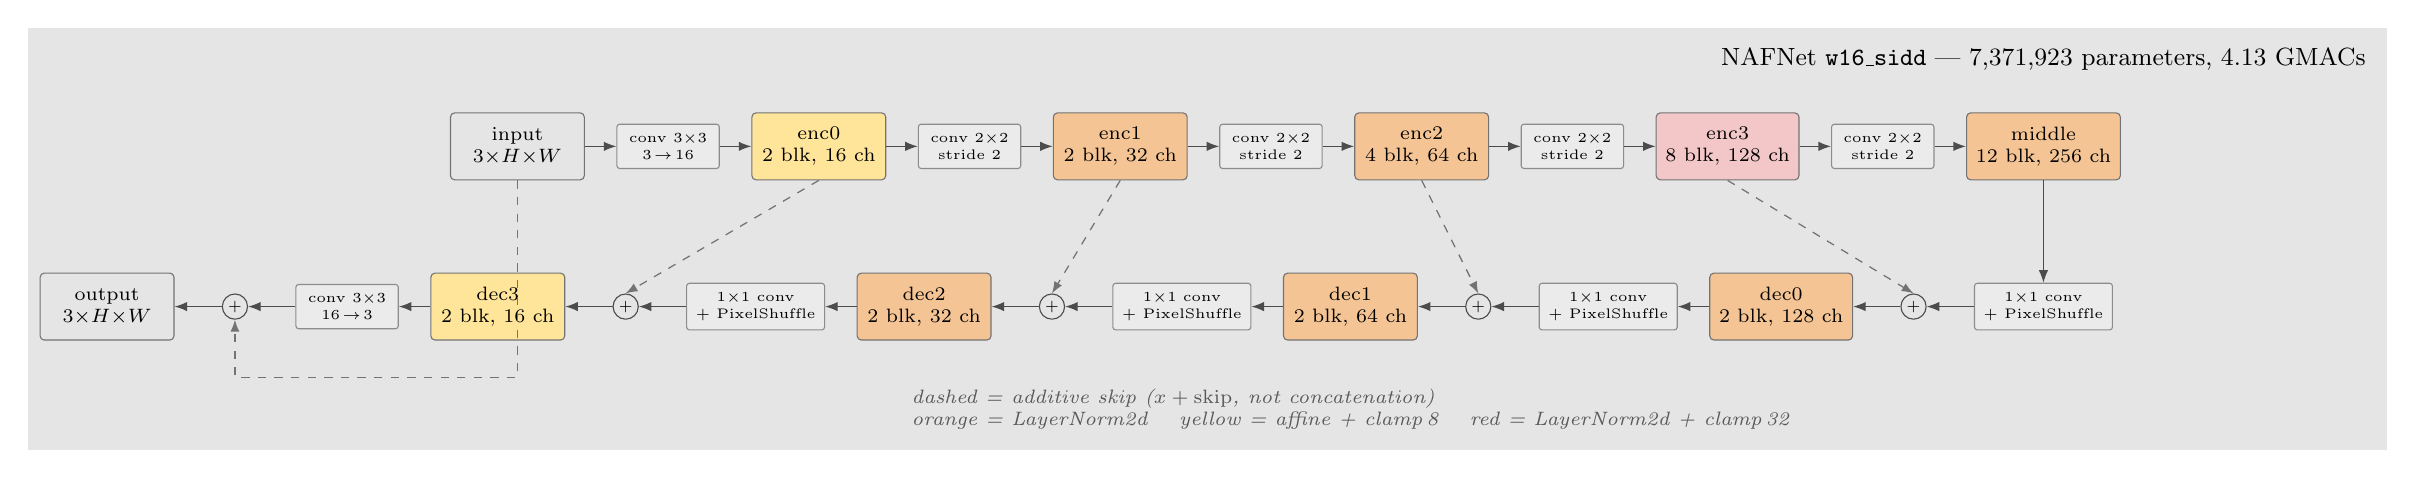
\begin{tikzpicture}[background rectangle/.style={fill=cBG},
                    show background rectangle, node distance=4mm]

  \node[stg, fill=black!10] (in)  at (0,0)   {input\\$3{\times}H{\times}W$};
  \node[resamp] (intro) [right=of in] {conv $3{\times}3$\\$3\!\to\!16$};

  % ---- encoder (colour = normalisation variant, per Figure 1) --------
  \node[stg, fill=cClamp] (e0) [right=of intro] {enc0\\2 blk, 16 ch};
  \node[resamp] (d0) [right=of e0] {conv $2{\times}2$\\stride 2};
  \node[stg, fill=cNorm]  (e1) [right=of d0] {enc1\\2 blk, 32 ch};
  \node[resamp] (d1) [right=of e1] {conv $2{\times}2$\\stride 2};
  \node[stg, fill=cNorm]  (e2) [right=of d1] {enc2\\4 blk, 64 ch};
  \node[resamp] (d2) [right=of e2] {conv $2{\times}2$\\stride 2};
  \node[stg, fill=cAttn!55] (e3) [right=of d2] {enc3\\8 blk, 128 ch};
  \node[resamp] (d3) [right=of e3] {conv $2{\times}2$\\stride 2};
  \node[stg, fill=cNorm]  (mid) [right=of d3] {middle\\12 blk, 256 ch};

  \foreach \a/\b in {in/intro, intro/e0, e0/d0, d0/e1, e1/d1, d1/e2,
                     e2/d2, d2/e3, e3/d3, d3/mid}
    \draw[flow] (\a) -- (\b);

  % ---- decoder, mirrored below --------------------------------------
  \node[resamp] (u0) [below=13mm of mid] {$1{\times}1$ conv\\ + PixelShuffle};
  \node[oplus]  (s0) [left=6mm of u0] {$+$};
  \node[stg, fill=cNorm] (c0) [left=6mm of s0] {dec0\\2 blk, 128 ch};
  \node[resamp] (u1) [left=of c0] {$1{\times}1$ conv\\ + PixelShuffle};
  \node[oplus]  (s1) [left=6mm of u1] {$+$};
  \node[stg, fill=cNorm] (c1) [left=6mm of s1] {dec1\\2 blk, 64 ch};
  \node[resamp] (u2) [left=of c1] {$1{\times}1$ conv\\ + PixelShuffle};
  \node[oplus]  (s2) [left=6mm of u2] {$+$};
  \node[stg, fill=cNorm] (c2) [left=6mm of s2] {dec2\\2 blk, 32 ch};
  \node[resamp] (u3) [left=of c2] {$1{\times}1$ conv\\ + PixelShuffle};
  \node[oplus]  (s3) [left=6mm of u3] {$+$};
  \node[stg, fill=cClamp] (c3) [left=6mm of s3] {dec3\\2 blk, 16 ch};
  \node[resamp] (endc) [left=of c3] {conv $3{\times}3$\\$16\!\to\!3$};
  \node[oplus]  (gres) [left=6mm of endc] {$+$};
  \node[stg, fill=black!10] (out) [left=6mm of gres] {output\\$3{\times}H{\times}W$};

  \draw[flow] (mid) -- (u0);
  \foreach \a/\b in {u0/s0, s0/c0, c0/u1, u1/s1, s1/c1, c1/u2, u2/s2,
                     s2/c2, c2/u3, u3/s3, s3/c3, c3/endc, endc/gres, gres/out}
    \draw[flow] (\a) -- (\b);

  % ---- ADDITIVE skips (x + skip, NOT concatenation) ------------------
  \foreach \e/\s in {e3/s0, e2/s1, e1/s2, e0/s3}
    \draw[skipl] (\e.south) -- (\s.north);
  % ---- global residual ----------------------------------------------
  \draw[skipl] (in.south) |- ($(gres)+(0,-9mm)$) -- (gres.south);

  \node[font=\scriptsize\itshape, text=black!65, align=left]
    at ($(c1)+(0,-13mm)$)
    {dashed = additive skip ($x+\mathrm{skip}$, not concatenation)\\
     orange = LayerNorm2d \quad yellow = affine + clamp\,8 \quad
     red = LayerNorm2d + clamp\,32};

  \node[font=\small] at ($(mid)+(0,11mm)$)
    {NAFNet \texttt{w16\_sidd} --- 7{,}371{,}923 parameters, 4.13 GMACs};

\end{tikzpicture}

\end{document}
